% SPDX-License-Identifier: CC-BY-NC-SA-3.0

% Copyright 2022 KUNBUS GmbH
% With work from https://git-scm.com/book/en/v2

\documentclass[aspectratio=169]{beamer}

\usepackage{minted}
\usepackage{xcolor}
\definecolor{LightGray}{gray}{0.9}

\usetheme {default}
\setbeamertemplate{navigation symbols}{}

\graphicspath{{images/}{\main/images/}}

% Title page details
\title {git training\footnote{This work is licensed under a \href{http://creativecommons.org/licenses/by-nc-sa/3.0/}{Creative Commons Attribution-NonCommercial-ShareAlike 3.0 Unported License.}}}
\subtitle{git, workflows, github}
\author{Philipp Rosenberger}
\institute{KUNBUS GmbH}
%\date{\today}

\renewcommand{\footnotesize}{\tiny}

\newcommand{\sectiontitle}{}
\newcommand{\newsection}[1]{\renewcommand{\sectiontitle}{#1}\section{#1}}

% Image Logo
\logo{
\includegraphics[width=2.5cm]{kunbus-logo.png}} 

\begin{document}

\begin{frame}
% Print the title page as the first slide
\titlepage
\end{frame}

% Presentation outline
\begin{frame}{Outline}
    \tableofcontents
\end{frame}

\section{What is a VCS?}
\begin{frame}{What is a VCS?}
\begin{itemize}
    \item Tracks changes
    \item Creates a history over the changes
    \item Provides traceability
    \item Provides attribution
\end{itemize}
\end{frame}

\begin{frame}{Centralized VCS}{Centralized vs. Distributed VCS}
\begin{figure}
    \centering
    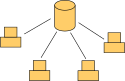
\includegraphics[width=\textwidth,height=0.6\textheight,keepaspectratio]{01_centralized_vcs}
\end{figure}
\end{frame}

\begin{frame}{Distributed VCS}{Centralized vs. Distributed VCS}
\begin{figure}
    \centering
    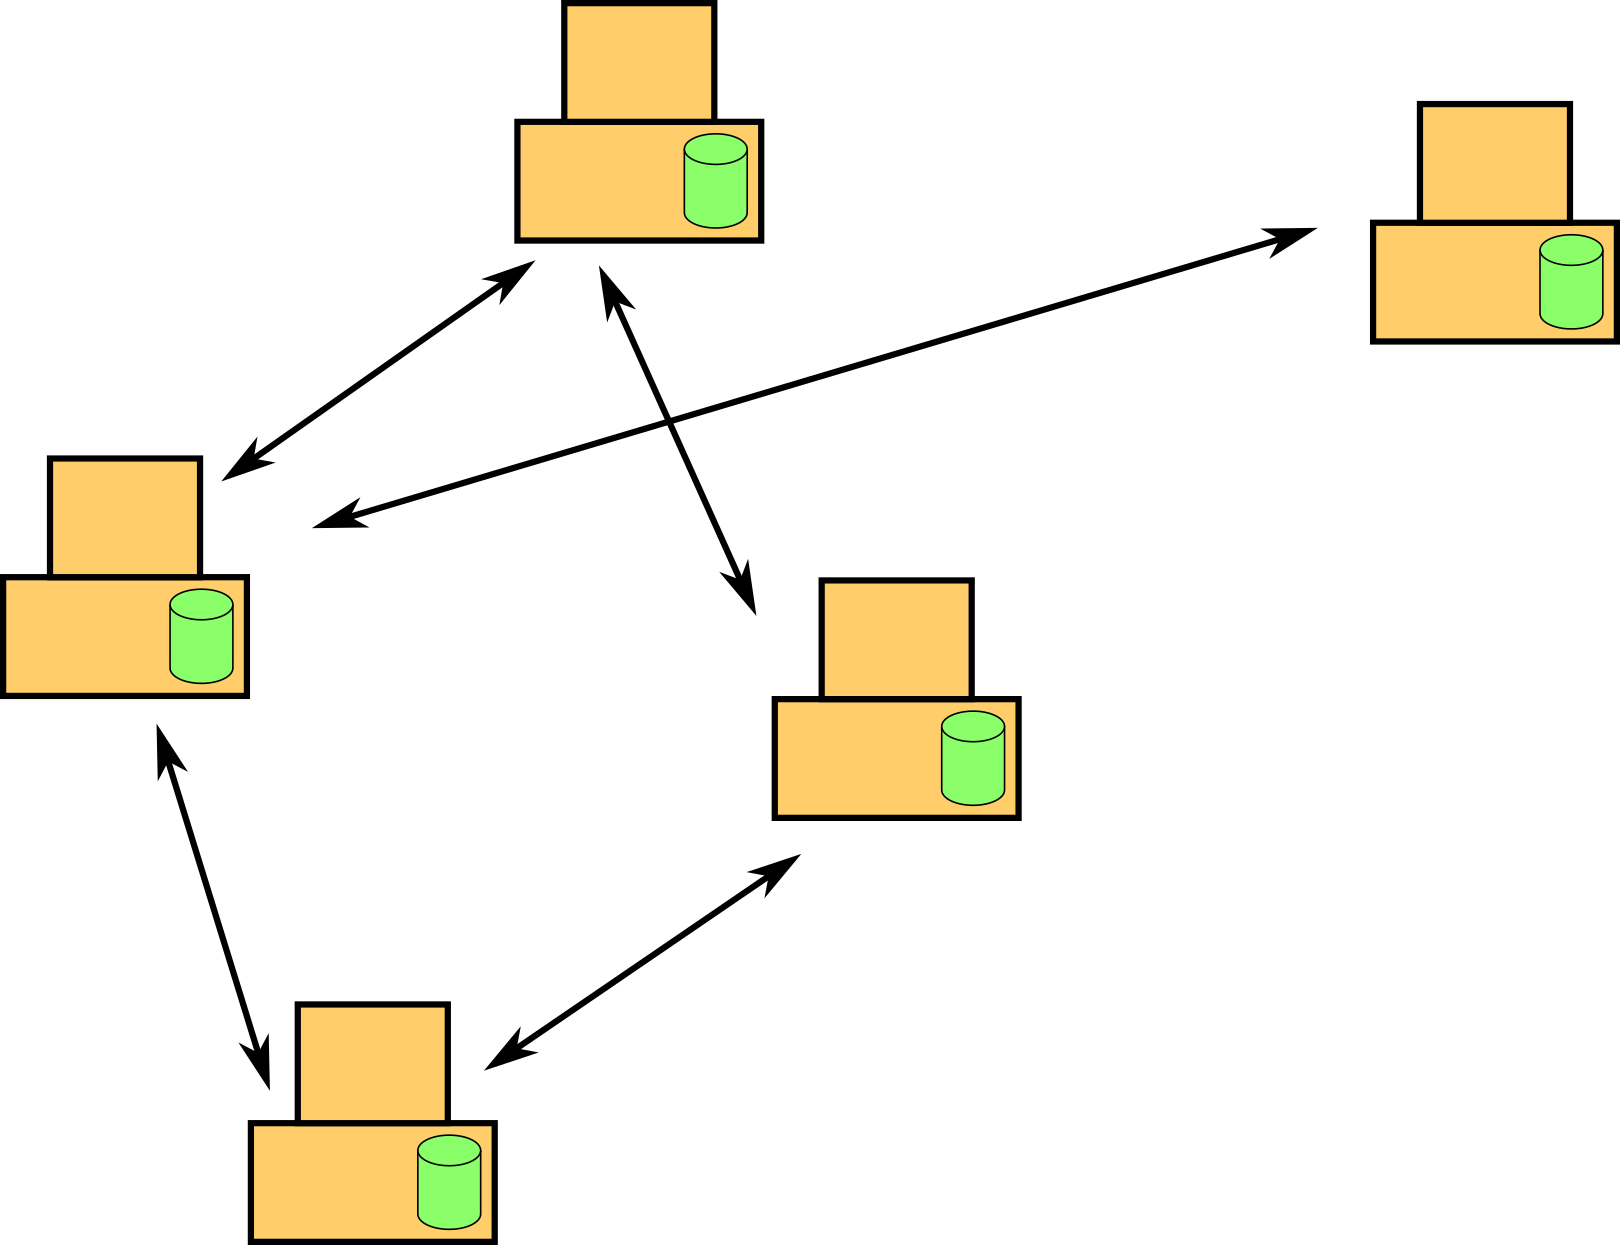
\includegraphics[width=\textwidth,height=0.6\textheight,keepaspectratio]{02_distributed_vcs}
\end{figure}
\end{frame}

\begin{frame}{Deltas}{Deltas vs. Snapshots}
\begin{figure}
    \centering
    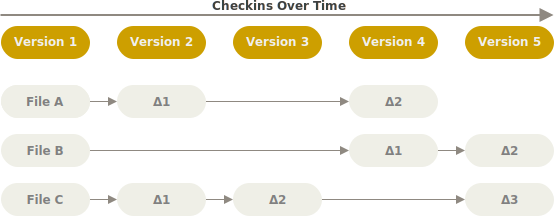
\includegraphics[width=\textwidth,height=0.6\textheight,keepaspectratio]{deltas}
    \caption{
        Storing data as changes to a base version of each file\footnote{
            Pro Git: 1.3 Getting Started - What is Git?
            (\url{https://git-scm.com/book/en/v2/Getting-Started-What-is-Git\%3F})
        }
    }
\end{figure}
\end{frame}

\begin{frame}{Snapshots}{Deltas vs. Snapshots}
\begin{figure}
    \centering
    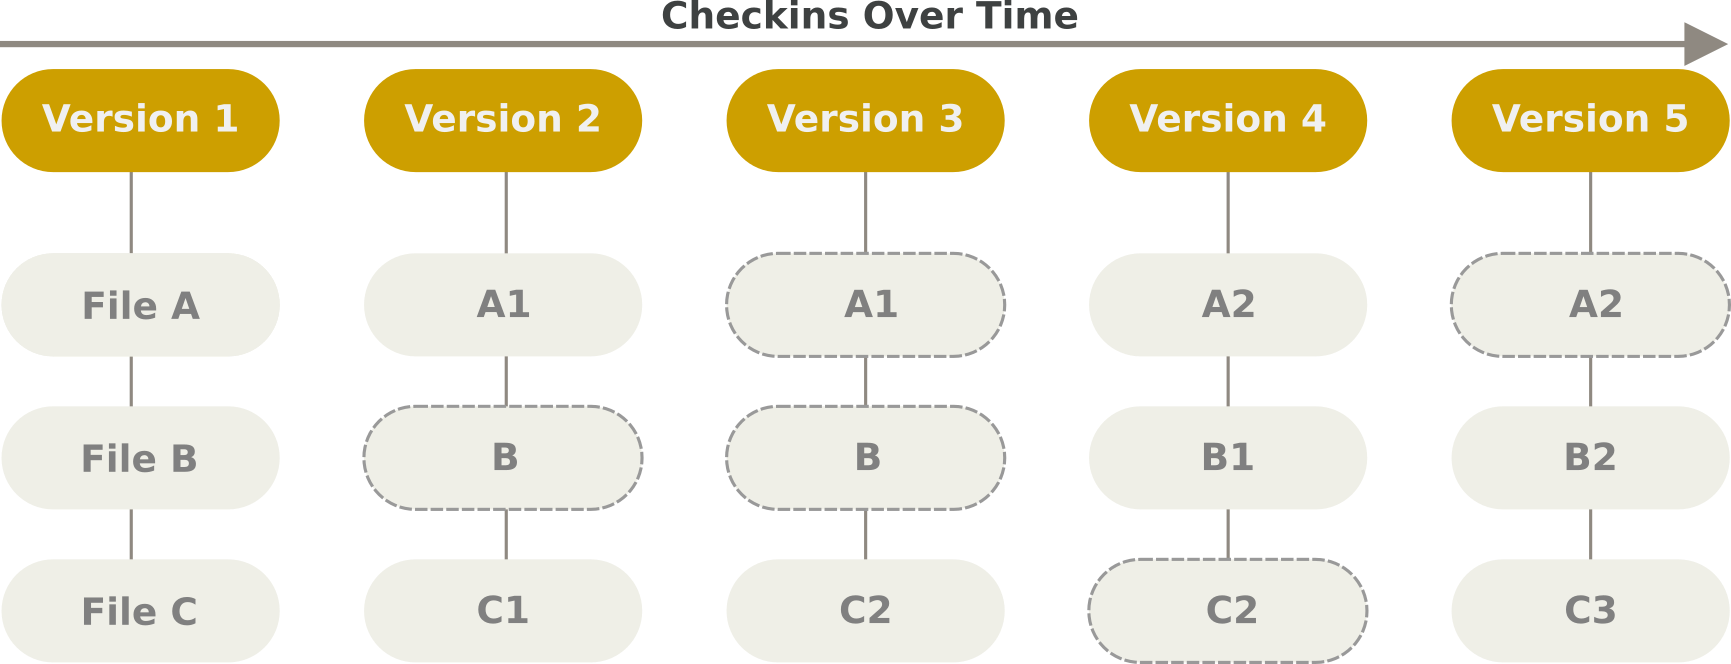
\includegraphics[width=\textwidth,height=0.6\textheight,keepaspectratio]{snapshots}
    \caption {
        Storing data as snapshots of the project over time\footnote{
            Pro Git: 1.3 Getting Started - What is Git?
            (\url{https://git-scm.com/book/en/v2/Getting-Started-What-is-Git\%3F})
        }
    }
\end{figure}
\end{frame}

\section{How does Git work?}
\begin{frame}[fragile]{Every thing is a Hash}{How does Git Work?}
\begin{minted}[bgcolor=LightGray,fontsize=\small]{text}
$ sha1sum kunbus-logo.png 
c263869cf482a5d5d4262170ec242f8f13fc3def  kunbus-logo.png
$ ls -sh kunbus-logo.png 
352K kunbus-logo.png
\end{minted}
\begin{itemize}
    \item A file is an \emph{object} with a \emph{hash} and a \emph{size}
    \item Everything is identified by its hash, not only file objects
\end{itemize}
\end{frame}

\begin{frame}{Git is a Tree of Hashes}{How does Git Work?}
\begin{figure}
    \centering
    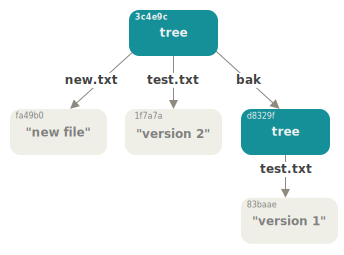
\includegraphics[width=\textwidth,height=0.6\textheight,keepaspectratio]{data-model-2}
    \caption{
        The content structure of your current Git data\footnote{
            Pro Git: 10.2 Git Internals - Git Objects
            (\url{https://git-scm.com/book/en/v2/Git-Internals-Git-Objects})
        }
    }
\end{figure}
\end{frame}

\begin{frame}{Git is a Tree of Trees of Hashes}{How does Git Work?}
\begin{figure}
    \centering
    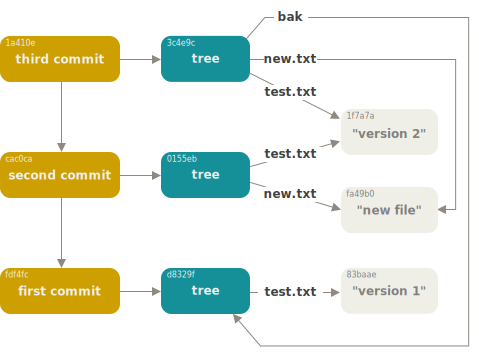
\includegraphics[width=\textwidth,height=0.6\textheight,keepaspectratio]{data-model-3}
    \caption{
        All the reachable objects in your Git directory\footnote{
            Pro Git: 10.2 Git Internals - Git Objects
            (\url{https://git-scm.com/book/en/v2/Git-Internals-Git-Objects})
        }
    }
\end{figure}
\end{frame}

\newsection{Git Basics}
\begin{frame}[fragile]{First-Time Git Setup}{\sectiontitle}
You need to configure your identity. If you ignore this step your commits will
have a wrong author. And I will not accept anything from you in my repository
or any company repository.
\begin{minted}[bgcolor=LightGray,fontsize=\small]{text}
$ git config --global user.name "John Doe"
$ git config --global user.email j.doe@kunbus.com
\end{minted}
You can also configure your preferred editor and customize git behavior:
\url{https://git-scm.com/book/en/v2/Getting-Started-First-Time-Git-Setup}
\end{frame}

\begin{frame}[fragile]{Getting a Git Repository}{\sectiontitle}
\begin{itemize}
    \item Create a directory
    \item Call \verb|git init| inside the directory
\end{itemize}
\begin{minted}[bgcolor=LightGray,fontsize=\small]{text}
$ mkdir my_project
$ cd my_project
$ git init
Initialized empty Git repository in /home/user/my_project/.git/
\end{minted}
\begin{itemize}
    \item This creates a local repository
    \item It is contained in the \verb|.git| directory under the \verb|my_project| directory
\end{itemize}
\end{frame}

\begin{frame}[fragile]{Getting a Git Repository}{\sectiontitle}
\begin{itemize}
    \item With \verb|git clone| we can get a remote repository
\end{itemize}
\begin{minted}[bgcolor=LightGray,fontsize=\small]{text}
$ git clone https://github.com/libgit2/libgit2
Cloning into 'libgit2'...
remote: Enumerating objects: 119184, done.
remote: Counting objects: 100% (119184/119184), done.
remote: Compressing objects: 100% (32744/32744), done.
remote: Total 119184 (delta 84532), reused 119074 (delta 84433), pack-r...
Receiving objects: 100% (119184/119184), 61.22 MiB | 7.21 MiB/s, done.
Resolving deltas: 100% (84532/84532), done.
\end{minted}
\begin{itemize}
    \item This creates the directory \verb|libgit2|
    \item A git repository (\verb|.git|) is create inside the directory
    \item The git repository contains a \emph{complete} copy of the remote repository
\end{itemize}
\end{frame}

\begin{frame}{Recording Changes to the Repository}{\sectiontitle}
\begin{block}{A file in your working tree can be in one (or more) of these for states}
    \begin{itemize}
        \item untracked
        \item unmodified
        \item modified
        \item staged
    \end{itemize}
\end{block}
\end{frame}

\begin{frame}{Recording Changes to the Repository}{\sectiontitle}
\begin{block}{untracked}
    Files which are in the working tree but are not under the control of git.
    They don't exist in the history. This can be new files or build artifacts
    which should not be included in the git repository.
\end{block}
\begin{block}{unmodified}
    Files which are under control of git. All changes have been recorded to the
    history. No additional changes have been made to the files.
\end{block}
\end{frame}


\begin{frame}{Recording Changes to the Repository}{\sectiontitle}
\begin{block}{modified}
    Files which are under control of git. Files that have been changed since
    the last time the changes to the file have been recorded to the history.
\end{block}
\begin{block}{staged}
    Files which are marked to be recorded to the history. Changes to files files
    in modified stage need to be staged before they can be recorded to the
    history. Also untracked files need to be staged before the can be recorded to
    the history.
\end{block}
\end{frame}

\begin{frame}{Recording Changes to the Repository}{\sectiontitle}
\begin{figure}
    \centering
    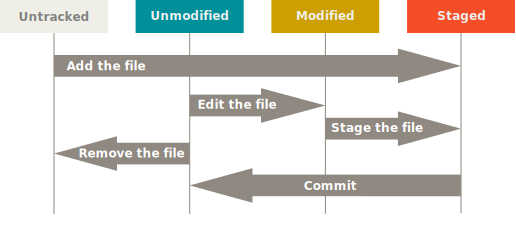
\includegraphics[width=\textwidth,height=0.6\textheight,keepaspectratio]{lifecycle}
    \caption{
        The lifecycle of the status of your files\footnote{
            Pro Git: 2.2 Git Basics - Recording Changes to the Repository
            (\url{https://git-scm.com/book/en/v2/Git-Basics-Recording-Changes-to-the-Repository})
        }
    }
\end{figure}
\end{frame}

\begin{frame}[fragile]{Recording Changes to the Repository}{\sectiontitle}
\begin{block}{Example: \ttfamily git add}
\begin{minted}[bgcolor=LightGray,fontsize=\footnotesize,breaklines]{text}
my_project$ echo "# My Project" > README.md
my_project$ git status 
On branch master

No commits yet

Untracked files:
  (use "git add <file>..." to include in what will be committed)
    README.md

nothing added to commit but untracked files present (use "git add" to track)
\end{minted}
\end{block}
\end{frame}

\begin{frame}[fragile]{Recording Changes to the Repository}{\sectiontitle}
\begin{block}{Example: \ttfamily git add}
\begin{minted}[bgcolor=LightGray,fontsize=\footnotesize]{text}
my_project$ git add README.md
my_project$ git status 
On branch master

No commits yet

Changes to be committed:
  (use "git rm --cached <file>..." to unstage)
    new file:   README.md
\end{minted}
\end{block}
\end{frame}

\begin{frame}[fragile]{Recording Changes to the Repository}{\sectiontitle}
\begin{block}{Example: \ttfamily git commit}
\begin{minted}[bgcolor=LightGray,fontsize=\footnotesize]{text}
my_project$ git commit
>EDITOR OPENS<
[master (root-commit) 1945062] Add initial REAMDE.md
 1 file changed, 1 insertion(+)
 create mode 100644 README.md
my_project$ git status
On branch master
nothing to commit, working tree clean
my_project$ ls
README.md
\end{minted}
\end{block}
\end{frame}

\begin{frame}[fragile]{Recording Changes to the Repository}{\sectiontitle}
\begin{block}{Example: Change file and commit changes}
\begin{minted}[bgcolor=LightGray,fontsize=\footnotesize]{text}
my_project$ echo -e "\nCopyright 2022 KUNBUS GmbH" >> README.md
my_project$ git status
On branch master
Changes not staged for commit:
  (use "git add <file>..." to update what will be committed)
  (use "git restore <file>..." to discard changes in working directory)
    modified:   README.md

no changes added to commit (use "git add" and/or "git commit -a")
my_project$ git add README.md
my_project$ git status 
On branch master
Changes to be committed:
  (use "git restore --staged <file>..." to unstage)
    modified:   README.md
my_project$ git commit
>EDITOR OPENS<
[master c16cceb] Add copyright
 1 file changed, 2 insertions(+)
\end{minted}
\end{block}
\end{frame}

\begin{frame}[fragile]{Recording Changes to the Repository}{\sectiontitle}
\begin{block}{Summary}
\begin{itemize}
    \item Add new files with \verb|git add| to the staging area
    \item Add changes with \verb|git add| to the staging area
    \item Use \verb|git status| to check the state of your files and working tree
    \item Use \verb|git commit| to record changes from the staging area to the history
\end{itemize}
\end{block}
\end{frame}

\begin{frame}[fragile]{Recording Changes to the Repository}{\sectiontitle}
\begin{block}{Exercise}
\begin{enumerate}
    \item Create a local git repository
    \item Create and add at least two files
    \item Commit your changes to the repository
    \item Make changes to one or more files
    \item Add and commit the changes
\end{enumerate}
\end{block}
\end{frame}

\begin{frame}[fragile]{Viewing the Commit History}{\sectiontitle}
\begin{block}{Example: \ttfamily git log}
\begin{minted}[bgcolor=LightGray,fontsize=\footnotesize]{text}
my_project$ git log
commit c16ccebd91c1a3d4b42cd575ad2912ef671ca506 (HEAD -> master)
Author: Philipp Rosenberger <p.rosenberger@kunbus.com>
Date:   Thu Dec 8 13:15:00 2022 +0100

    Add copyright

commit 19450627f83f4e51ad42ece86d9d2a5279bc2c23
Author: Philipp Rosenberger <p.rosenberger@kunbus.com>
Date:   Wed Dec 7 13:15:11 2022 +0100

    Add initial REAMDE.md
    
    Add a README.md file with just the project name as starting point

\end{minted}
\end{block}
\end{frame}

\begin{frame}[fragile]{Viewing the Commit History}{\sectiontitle}
\begin{block}{Example: \ttfamily git log --pretty=fuller}
\begin{minted}[bgcolor=LightGray,fontsize=\footnotesize]{text}
my_project$ git log --pretty=fuller 
commit c16ccebd91c1a3d4b42cd575ad2912ef671ca506 (HEAD -> master)
Author:     Philipp Rosenberger <p.rosenberger@kunbus.com>
AuthorDate: Thu Dec 8 13:15:00 2022 +0100
Commit:     Philipp Rosenberger <p.rosenberger@kunbus.com>
CommitDate: Thu Dec 8 14:00:34 2022 +0100

    Add copyright

commit 19450627f83f4e51ad42ece86d9d2a5279bc2c23
Author:     Philipp Rosenberger <p.rosenberger@kunbus.com>
AuthorDate: Wed Dec 7 13:15:11 2022 +0100
Commit:     Philipp Rosenberger <p.rosenberger@kunbus.com>
CommitDate: Thu Dec 8 14:00:29 2022 +0100

    Add initial REAMDE.md
    
    Add a README.md file with just the project name as starting point
\end{minted}
\end{block}
\end{frame}

\begin{frame}[fragile]{Viewing the Commit History}{\sectiontitle}
\begin{block}{Example: \ttfamily git show}
\begin{minted}[bgcolor=LightGray,fontsize=\footnotesize]{diff}
my_project$ git show 19450627f83f4e51ad42ece86d9d2a5279bc2c23
commit 19450627f83f4e51ad42ece86d9d2a5279bc2c23
Author: Philipp Rosenberger <p.rosenberger@kunbus.com>
Date:   Wed Dec 7 13:15:11 2022 +0100

    Add initial REAMDE.md
    
    Add a README.md file with just the project name as starting point

diff --git a/README.md b/README.md
new file mode 100644
index 0000000..a2beefd
--- /dev/null
+++ b/README.md
@@ -0,0 +1 @@
+# My Project
\end{minted}
\end{block}
\end{frame}

\begin{frame}[fragile]{Viewing the Commit History}{\sectiontitle}
\begin{block}{Summary}
\begin{itemize}
    \item List the history with \verb|git log|
    \item The difference between author and committer 
    \item Inspect any commit form you history (or git repo) with \verb|git show|
\end{itemize}
\end{block}
\end{frame}

\begin{frame}[fragile]{Undoing Things}{\sectiontitle}
\begin{block}{Example: Change your last commit: \texttt{git commit --amend} {\small(1)}}
\begin{minted}[bgcolor=LightGray,fontsize=\footnotesize]{diff}
my_project$ vim README.md
my_project$ git diff
diff --git a/README.md b/README.md
index 7207d0d..272997d 100644
--- a/README.md
+++ b/README.md
@@ -1,3 +1,3 @@
 # My Project
 
-Copyright 2022 KUNBUS GmbH
+Copyright 2022 KUNBUS GmbH <support@kunbus.com>
my_project$ git status 
On branch master
Changes not staged for commit:
  (use "git add <file>..." to update what will be committed)
  (use "git restore <file>..." to discard changes in working directory)
    modified:   README.md

no changes added to commit (use "git add" and/or "git commit -a")
\end{minted}
\end{block}
\end{frame}

\begin{frame}[fragile]{Undoing Things}{\sectiontitle}
\begin{block}{Example: Change your last commit: \texttt{git commit --amend} {\small(2)}}
\begin{minted}[bgcolor=LightGray,fontsize=\footnotesize]{diff}
my_project$ git add README.md
my_project$ git status 
On branch master
Changes to be committed:
  (use "git restore --staged <file>..." to unstage)
    modified:   README.md

my_project$ git commit --amend
>EDITOR OPENS<
[master 0e59905] Add KUNBUS copyright notice
 Date: Thu Dec 8 13:15:00 2022 +0100
 1 file changed, 2 insertions(+)
\end{minted}
\end{block}
\end{frame}

\begin{frame}[fragile]{Undoing Things}{\sectiontitle}
\begin{block}{Example: Change your last commit: \texttt{git commit --amend} {\small(3)}}
\begin{minted}[bgcolor=LightGray,fontsize=\footnotesize]{diff}
my_project$ git show HEAD
commit 0e59905d83e2d075098d0ea3d0ec4c4f2b45bbfc (HEAD -> master)
Author: Philipp Rosenberger <p.rosenberger@kunbus.com>
Date:   Thu Dec 8 13:15:00 2022 +0100

    Add KUNBUS copyright notice

diff --git a/README.md b/README.md
index a2beefd..272997d 100644
--- a/README.md
+++ b/README.md
@@ -1 +1,3 @@
 # My Project
+
+Copyright 2022 KUNBUS GmbH <support@kunbus.com>
\end{minted}
\end{block}
\end{frame}

\begin{frame}[fragile]{Undoing Things}{\sectiontitle}
\begin{block}{Example: Change your last commit: \texttt{git commit --amend} {\small(4)}}
\begin{minted}[bgcolor=LightGray,fontsize=\footnotesize]{text}
my_project$ git log
commit 0e59905d83e2d075098d0ea3d0ec4c4f2b45bbfc (HEAD -> master)
Author: Philipp Rosenberger <p.rosenberger@kunbus.com>
Date:   Thu Dec 8 13:15:00 2022 +0100

    Add KUNBUS copyright notice

commit 19450627f83f4e51ad42ece86d9d2a5279bc2c23
Author: Philipp Rosenberger <p.rosenberger@kunbus.com>
Date:   Wed Dec 7 13:15:11 2022 +0100

    Add initial REAMDE.md
    
    Add a README.md file with just the project name as starting point
\end{minted}
\end{block}
\end{frame}

\begin{frame}[fragile]{Undoing Things}{\sectiontitle}
\begin{block}{Summary}
\begin{itemize}
    \item Change the last commit with \verb|git commit --amend|
    \item The key word \verb|HEAD| references the current (last) commit in the work tree
\end{itemize}
\end{block}
\end{frame}

\begin{frame}[fragile]{Undoing Things}{\sectiontitle}
\begin{block}{Exercise}
Use your repository from the last exercise.
\begin{enumerate}
    \item List the history of you repository
    \item Inspect the first/initial commit
    \item Change the last commit of your history
\end{enumerate}
\end{block}
\end{frame}

\newsection{Git Branching}
\begin{frame}{Branches in a Nutshell}{\sectiontitle}
\begin{figure}
    \centering
    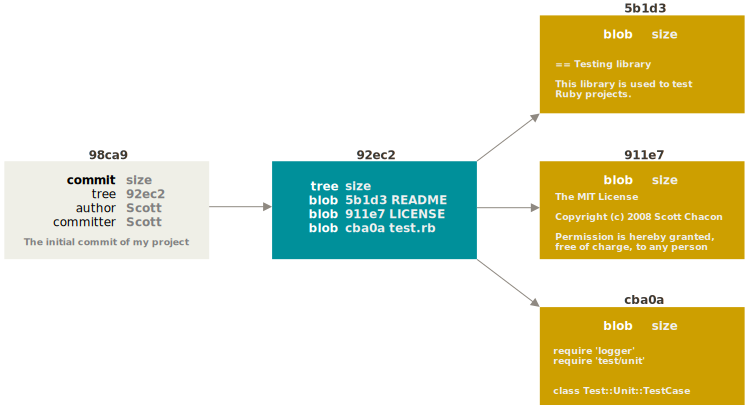
\includegraphics[width=\textwidth,height=0.6\textheight,keepaspectratio]{commit-and-tree}
    \caption{
        A Commit and its tree\footnote{
            Pro Git: 3.1 Git Branching - Branches in a Nutshell
            (\url{https://git-scm.com/book/en/v2/Git-Branching-Branches-in-a-Nutshell})
        }
    }
\end{figure}
\end{frame}

\begin{frame}{Branches in a Nutshell}{\sectiontitle}
\begin{figure}
    \centering
    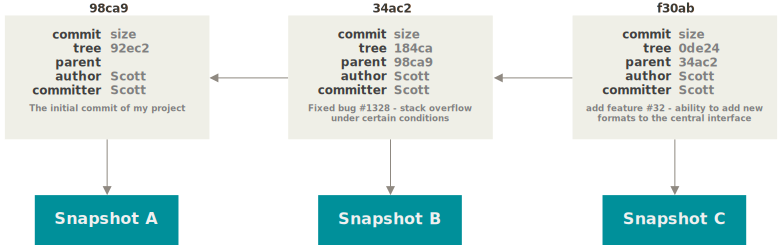
\includegraphics[width=\textwidth,height=0.6\textheight,keepaspectratio]{commits-and-parents}
    \caption{
        Commits and their parents\footnote{
            Pro Git: 3.1 Git Branching - Branches in a Nutshell
            (\url{https://git-scm.com/book/en/v2/Git-Branching-Branches-in-a-Nutshell})
        }
    }
\end{figure}
\end{frame}

\begin{frame}[fragile]{Branches in a Nutshell}{\sectiontitle}
\begin{minted}[bgcolor=LightGray,fontsize=\footnotesize]{diff}
$ git branch testing
\end{minted}
\begin{figure}
    \centering
    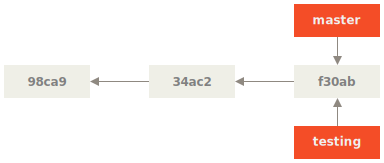
\includegraphics[width=\textwidth,height=0.5\textheight,keepaspectratio]{two-branches}
    \caption{
        Two branches pointing into the same series of commits\footnote{
            Pro Git: 3.1 Git Branching - Branches in a Nutshell
            (\url{https://git-scm.com/book/en/v2/Git-Branching-Branches-in-a-Nutshell})
        }
    }
\end{figure}
\end{frame}

\begin{frame}{Branches in a Nutshell}{\sectiontitle}
\begin{figure}
    \centering
    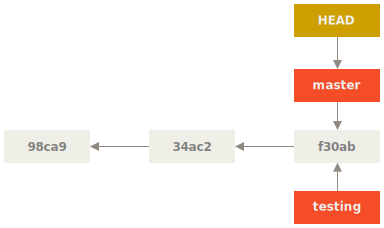
\includegraphics[width=\textwidth,height=0.6\textheight,keepaspectratio]{head-to-master}
    \caption{
        HEAD pointing to a branch\footnote{
            Pro Git: 3.1 Git Branching - Branches in a Nutshell
            (\url{https://git-scm.com/book/en/v2/Git-Branching-Branches-in-a-Nutshell})
        }
    }
\end{figure}
\end{frame}

\begin{frame}[fragile]{Branches in a Nutshell}{\sectiontitle}
\begin{minted}[bgcolor=LightGray,fontsize=\footnotesize]{diff}
$ git checkout testing
\end{minted}
\begin{figure}
    \centering
    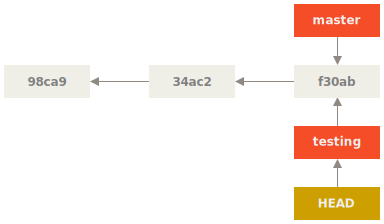
\includegraphics[width=\textwidth,height=0.5\textheight,keepaspectratio]{head-to-testing}
    \caption{
        HEAD points to the current branch\footnote{
            Pro Git: 3.1 Git Branching - Branches in a Nutshell
            (\url{https://git-scm.com/book/en/v2/Git-Branching-Branches-in-a-Nutshell})
        }
    }
\end{figure}
\end{frame}

\begin{frame}[fragile]{Branches in a Nutshell}{\sectiontitle}
\begin{minted}[bgcolor=LightGray,fontsize=\footnotesize]{diff}
$ vim test.rb
$ git commit -a -m 'made a change'
\end{minted}
\begin{figure}
    \centering
    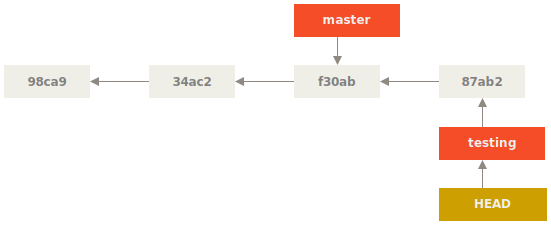
\includegraphics[width=\textwidth,height=0.5\textheight,keepaspectratio]{advance-testing}
    \caption{
        The HEAD branch moves forward when a commit is made\footnote{
            Pro Git: 3.1 Git Branching - Branches in a Nutshell
            (\url{https://git-scm.com/book/en/v2/Git-Branching-Branches-in-a-Nutshell})
        }
    }
\end{figure}
\end{frame}

\begin{frame}[fragile]{Branches in a Nutshell}{\sectiontitle}
\begin{minted}[bgcolor=LightGray,fontsize=\footnotesize]{diff}
$ git checkout master
\end{minted}
\begin{figure}
    \centering
    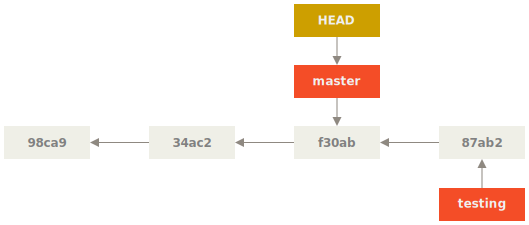
\includegraphics[width=\textwidth,height=0.5\textheight,keepaspectratio]{checkout-master}
    \caption{
        HEAD moves when you checkout\footnote{
            Pro Git: 3.1 Git Branching - Branches in a Nutshell
            (\url{https://git-scm.com/book/en/v2/Git-Branching-Branches-in-a-Nutshell})
        }
    }
\end{figure}
\end{frame}

\begin{frame}[fragile]{Branches in a Nutshell}{\sectiontitle}
\begin{minted}[bgcolor=LightGray,fontsize=\footnotesize]{diff}
$ vim test.rb
$ git commit -a -m 'made other changes'
\end{minted}
\begin{figure}
    \centering
    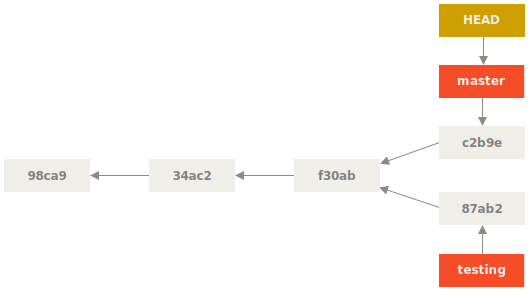
\includegraphics[width=\textwidth,height=0.5\textheight,keepaspectratio]{advance-master}
    \caption{
        Divergent history\footnote{
            Pro Git: 3.1 Git Branching - Branches in a Nutshell
            (\url{https://git-scm.com/book/en/v2/Git-Branching-Branches-in-a-Nutshell})
        }
    }
\end{figure}
\end{frame}

\begin{frame}{Basic Branching and Merging}{\sectiontitle}
\begin{figure}
    \centering
    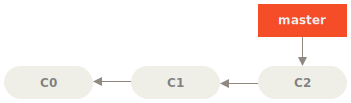
\includegraphics[width=\textwidth,height=0.5\textheight,keepaspectratio]{basic-branching-1}
    \caption{
        A simple commit history\footnote{
            Pro Git: 3.2 Git Branching - Basic Branching and Merging
            (\url{https://git-scm.com/book/en/v2/Git-Branching-Basic-Branching-and-Merging})
        }
    }
\end{figure}
\end{frame}

\begin{frame}[fragile]{Basic Branching and Merging}{\sectiontitle}
\begin{minted}[bgcolor=LightGray,fontsize=\footnotesize]{diff}
$ git checkout -b iss53
\end{minted}
\begin{figure}
    \centering
    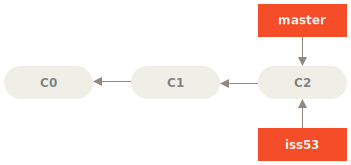
\includegraphics[width=\textwidth,height=0.5\textheight,keepaspectratio]{basic-branching-2}
    \caption{
        Creating a new branch pointer\footnote{
            Pro Git: 3.2 Git Branching - Basic Branching and Merging
            (\url{https://git-scm.com/book/en/v2/Git-Branching-Basic-Branching-and-Merging})
        }
    }
\end{figure}
\end{frame}

\begin{frame}[fragile]{Basic Branching and Merging}{\sectiontitle}
\begin{minted}[bgcolor=LightGray,fontsize=\footnotesize]{diff}
$ vim index.html
$ git commit -a -m 'Create new footer [issue 53]'
\end{minted}
\begin{figure}
    \centering
    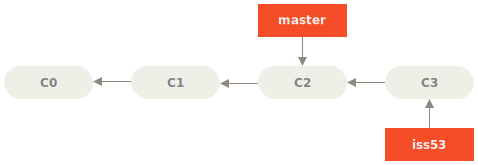
\includegraphics[width=\textwidth,height=0.5\textheight,keepaspectratio]{basic-branching-3}
    \caption{
        The \texttt{iss53} branch has moved forward with your work\footnote{
            Pro Git: 3.2 Git Branching - Basic Branching and Merging
            (\url{https://git-scm.com/book/en/v2/Git-Branching-Basic-Branching-and-Merging})
        }
    }
\end{figure}
\end{frame}

\begin{frame}[fragile]{Basic Branching and Merging}{\sectiontitle}
There is an issue with your code in the \texttt{master} branch. You need to
create a hotfix for this. So we switch back to the master branch.
\begin{minted}[bgcolor=LightGray,fontsize=\footnotesize]{diff}
$ git checkout master
Switched to branch 'master'
\end{minted}
And now we create a \texttt{hotfix} branch. And create a commit to fix the broken
email address.
\begin{minted}[bgcolor=LightGray,fontsize=\footnotesize]{diff}
$ git checkout -b hotfix master
Switched to a new branch 'hotfix'
$ vim index.html
$ git commit -a -m 'Fix broken email address'
[hotfix 1fb7853] Fix broken email address
 1 file changed, 2 insertions(+)
\end{minted}
\end{frame}

\begin{frame}[fragile]{Basic Branching and Merging}{\sectiontitle}
\begin{figure}
    \centering
    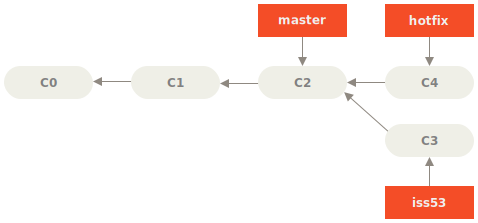
\includegraphics[width=\textwidth,height=0.5\textheight,keepaspectratio]{basic-branching-4}
    \caption{
        Hotfix branch based on \texttt{master}\footnote{
            Pro Git: 3.2 Git Branching - Basic Branching and Merging
            (\url{https://git-scm.com/book/en/v2/Git-Branching-Basic-Branching-and-Merging})
        }
    }
\end{figure}
\end{frame}

\begin{frame}[fragile]{Basic Branching and Merging}{\sectiontitle}
Now we need to merge the \texttt{hotfix} branch into our \texttt{master} branch.
\begin{minted}[bgcolor=LightGray,fontsize=\footnotesize]{diff}
$ git checkout master
$ git merge hotfix
Updating f42c576..3a0874c
Fast-forward
 index.html | 2 ++
 1 file changed, 2 insertions(+)
\end{minted}
\end{frame}

\begin{frame}[fragile]{Basic Branching and Merging}{\sectiontitle}
\begin{figure}
    \centering
    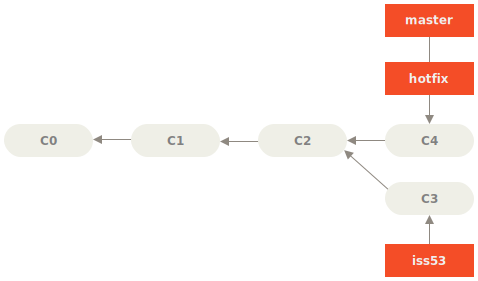
\includegraphics[width=\textwidth,height=0.5\textheight,keepaspectratio]{basic-branching-5}
    \caption{
        \texttt{master} is \emph{fast-forwarded} to \texttt{hotfix}\footnote{
            Pro Git: 3.2 Git Branching - Basic Branching and Merging
            (\url{https://git-scm.com/book/en/v2/Git-Branching-Basic-Branching-and-Merging})
        }
    }
\end{figure}
\end{frame}

\begin{frame}[fragile]{Basic Branching and Merging}{\sectiontitle}
Delete the \verb|hotfix| branch.
\begin{minted}[bgcolor=LightGray,fontsize=\footnotesize]{diff}
$ git branch -d hotfix
Deleted branch hotfix (3a0874c).
\end{minted}
Switch back to the \verb|iss53| branch to continue your work.
\begin{minted}[bgcolor=LightGray,fontsize=\footnotesize]{diff}
$ git checkout iss53
Switched to branch "iss53"
$ vim index.html
$ git commit -a -m 'Finish the new footer [issue 53]'
[iss53 ad82d7a] Finish the new footer [issue 53]
1 file changed, 1 insertion(+)
\end{minted}
\end{frame}

\begin{frame}[fragile]{Basic Branching and Merging}{\sectiontitle}
\begin{figure}
    \centering
    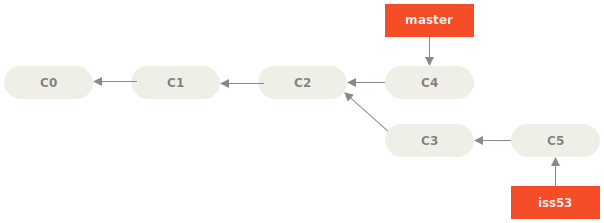
\includegraphics[width=\textwidth,height=0.5\textheight,keepaspectratio]{basic-branching-6}
    \caption{
        Work continues on \texttt{iss53}\footnote{
            Pro Git: 3.2 Git Branching - Basic Branching and Merging
            (\url{https://git-scm.com/book/en/v2/Git-Branching-Basic-Branching-and-Merging})
        }
    }
\end{figure}
\end{frame}

\begin{frame}[fragile]{Basic Branching and Merging}{\sectiontitle}
The feature on the \verb|iss53| is done and can be merged into the master branch.
\begin{minted}[bgcolor=LightGray,fontsize=\footnotesize]{diff}
$ git checkout master
Switched to branch 'master'
$ git merge iss53
Merge made by the 'recursive' strategy.
index.html |    1 +
1 file changed, 1 insertion(+)
\end{minted}
\end{frame}

\begin{frame}[fragile]{Basic Branching and Merging}{\sectiontitle}
\begin{figure}
    \centering
    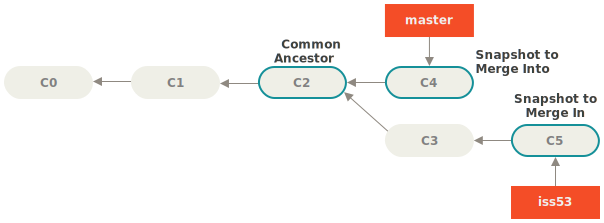
\includegraphics[width=\textwidth,height=0.5\textheight,keepaspectratio]{basic-merging-1}
    \caption{
         Three snapshots used in a typical merge\footnote{
            Pro Git: 3.2 Git Branching - Basic Branching and Merging
            (\url{https://git-scm.com/book/en/v2/Git-Branching-Basic-Branching-and-Merging})
        }
    }
\end{figure}
\end{frame}

\begin{frame}[fragile]{Basic Branching and Merging}{\sectiontitle}
\begin{figure}
    \centering
    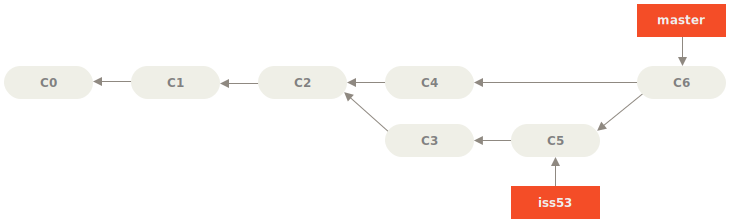
\includegraphics[width=\textwidth,height=0.5\textheight,keepaspectratio]{basic-merging-2}
    \caption{
         A merge commit\footnote{
            Pro Git: 3.2 Git Branching - Basic Branching and Merging
            (\url{https://git-scm.com/book/en/v2/Git-Branching-Basic-Branching-and-Merging})
        }
    }
\end{figure}
\end{frame}

\begin{frame}[fragile]{Basic Branching and Merging}{\sectiontitle}
\begin{block}{Merge Conflicts}
When merging two branches which made changes to the same code it is likely you will get a merge conflict.
\begin{minted}[bgcolor=LightGray,fontsize=\footnotesize]{diff}
$ git merge iss53
Auto-merging index.html
CONFLICT (content): Merge conflict in index.html
Automatic merge failed; fix conflicts and then commit the result.
$ git status
On branch master
You have unmerged paths.
  (fix conflicts and run "git commit")

Unmerged paths:
  (use "git add <file>..." to mark resolution)

    both modified:      index.html

no changes added to commit (use "git add" and/or "git commit -a")
\end{minted}
\end{block}
\end{frame}

\begin{frame}[fragile]{Basic Branching and Merging}{\sectiontitle}
\begin{block}{Summary}
\begin{itemize}
    \item Creating branches with \verb|git branch| or \verb|git checkout -b|
    \item Switching between branches with \verb|git checkout|
    \item Merging branches with \verb|git merge|
    \item The difference between a merge commit and a fast-forward merge
    \item Deleting branches with \verb|git branch -d|
\end{itemize}
\end{block}
\end{frame}

\newsection{Working with Remotes}
\begin{frame}{What is a remote (repository)?}{\sectiontitle}
\begin{itemize}
    \item A remote repository is separate repository
    \item It is most likely accessed over the network (e.g. ssh, https, \ldots)
    \item It is configured in your local repository as \emph{remote}
\end{itemize}
\end{frame}

\begin{frame}[fragile]{What is a remote (repository)?}{\sectiontitle}
\begin{block}{\texttt{git clone}}
The simplest and most common way to configure a remote is to \emph{clone} a
remote git repository. We have already discussed this.
\begin{minted}[bgcolor=LightGray,fontsize=\footnotesize]{text}
$ git clone https://github.com/schacon/ticgit
Cloning into 'ticgit'...
remote: Reusing existing pack: 1857, done.
remote: Total 1857 (delta 0), reused 0 (delta 0)
Receiving objects: 100% (1857/1857), 374.35 KiB | 268.00 KiB/s, done.
Resolving deltas: 100% (772/772), done.
Checking connectivity... done.
$ cd ticgit
$ git remote -v
origin	https://github.com/schacon/ticgit (fetch)
origin	https://github.com/schacon/ticgit (push)
\end{minted}
\end{block}
\end{frame}

\begin{frame}[fragile]{What is a remote (repository)?}{\sectiontitle}
\begin{block}{What's up with this \texttt{origin}?}
\begin{itemize}
    \item When you clone a repo the remote (from where you cloned it) will be called origin
    \item You can rename it as you like
\end{itemize}
\end{block}
\begin{minted}[bgcolor=LightGray,fontsize=\footnotesize]{text}
$ git remote rename origin schacon
$ git remote -v
schacon	https://github.com/schacon/ticgit (fetch)
schacon	https://github.com/schacon/ticgit (push)
\end{minted}
\end{frame}

\begin{frame}[fragile]{Multiple Remotes}{\sectiontitle}
\begin{block}{How to add a remote?}
You can have as many remotes as you like/need. Use \verb|git remote add| to
add a new remote:
\begin{minted}[bgcolor=LightGray,fontsize=\footnotesize]{text}
$ git remote add ilu git@github.com:iluminat23/ticgit.git
$ git remote -v
ilu	git@github.com:iluminat23/ticgit.git (fetch)
ilu	git@github.com:iluminat23/ticgit.git (push)
schacon	https://github.com/schacon/ticgit (fetch)
schacon	https://github.com/schacon/ticgit (push)
\end{minted}
\begin{itemize}
    \item The first remote (\verb|ilu|) is using ssh
    \item The second remote (\verb|schacon|) is using https
\end{itemize}
\end{block}
\end{frame}

\begin{frame}[fragile]{Multiple Remotes}{\sectiontitle}
\begin{block}{How to add a remote?}
When you create a local git repo it has no remotes. But you can add a remote any time.
\begin{minted}[bgcolor=LightGray,fontsize=\footnotesize]{text}
$ mkdir empty_repo
$ cd empty_repo/
$ git init
Initialized empty Git repository in /tmp/empty_repo/.git/
$ git remote -v
$ git remote add ilu git@github.com:iluminat23/example_repo.git
$ git remote -v
ilu	git@github.com:iluminat23/example_repo.git (fetch)
ilu	git@github.com:iluminat23/example_repo.git (push)
\end{minted}
\end{block}
\end{frame}

\begin{frame}[fragile]{Multiple Remotes}{\sectiontitle}
\begin{block}{How to synchronize the local repo?}
To get the (newest) data from a remote use \verb|git fetch|.
\begin{minted}[bgcolor=LightGray,fontsize=\footnotesize]{text}
$ mkdir ticgit && cd ticgit/
$ git init
$ git remote add ilu git@github.com:iluminat23/ticgit.git
$ git fetch ilu
remote: Enumerating objects: 1827, done.
remote: Total 1827 (delta 0), reused 0 (delta 0), pack-reused 1827
Receiving objects: 100% (1827/1827), 328.07 KiB | 1.09 MiB/s, done.
Resolving deltas: 100% (828/828), done.
From github.com:iluminat23/ticgit
 * [new branch]      master     -> ilu/master
\end{minted}
\end{block}
\end{frame}

\begin{frame}[fragile]{Remote Branches}{\sectiontitle}
\begin{itemize}
    \item Remote references are references (pointers) in your remote repositories
    \item Remote-tracking branches are references to the state of remote branches
    \item Remote-tracking branch names take the form \verb|<remote>/<branch>| (e.g. \verb|origin/master|)
\end{itemize}
\end{frame}

\begin{frame}[fragile]{Remote Branches}{\sectiontitle}
\begin{block}{Example}
\begin{itemize}
    \item Your git server is \verb|git.ourcompany.com|
    \item You cloned the repo and the remote is named \verb|origin|
    \item Development happens on the \verb|master| branch
\end{itemize}
\end{block}
\end{frame}

\begin{frame}{Remote Branches}{\sectiontitle}
\begin{figure}
    \centering
    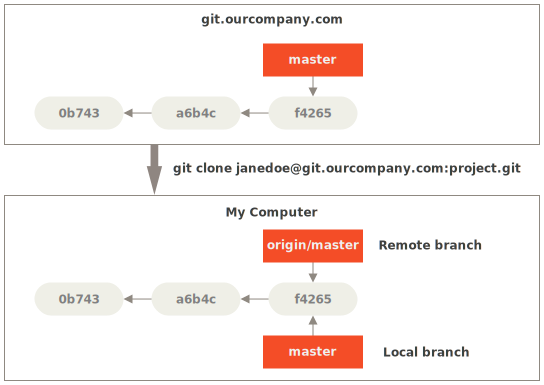
\includegraphics[width=\textwidth,height=0.5\textheight,keepaspectratio]{remote-branches-1}
    \caption{
        Server and local repositories after cloning\footnote{
            3.5 Git Branching - Remote Branches
            (\url{https://git-scm.com/book/en/v2/Git-Branching-Remote-Branches})
        }
    }
\end{figure}
\end{frame}

\begin{frame}[fragile]{Remote Branches}{\sectiontitle}
\begin{itemize}
    \item You do some work on your local \verb|master|
    \item Someone else does some work on the remote \verb|master|
\end{itemize}
\end{frame}

\begin{frame}{Remote Branches}{\sectiontitle}
\begin{figure}
    \centering
    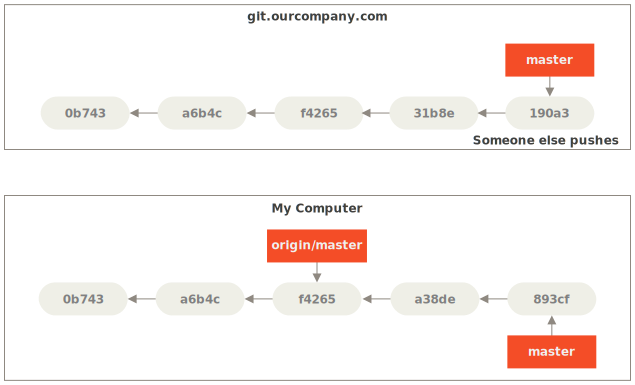
\includegraphics[width=\textwidth,height=0.5\textheight,keepaspectratio]{remote-branches-2}
    \caption{
        Local and remote work can diverge\footnote{
            3.5 Git Branching - Remote Branches
            (\url{https://git-scm.com/book/en/v2/Git-Branching-Remote-Branches})
        }
    }
\end{figure}
\end{frame}

\begin{frame}{Remote Branches}{\sectiontitle}
\begin{figure}
    \centering
    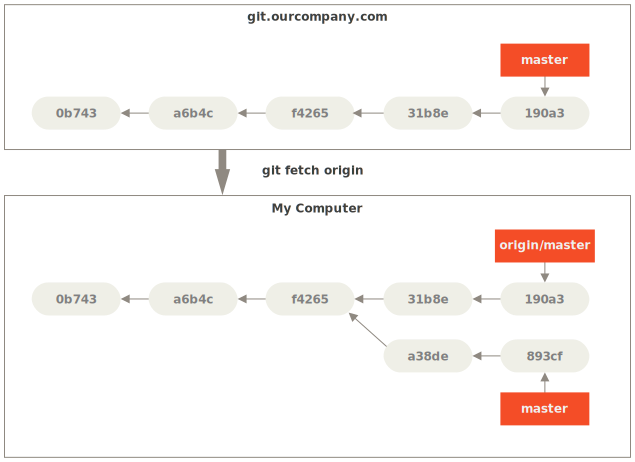
\includegraphics[width=\textwidth,height=0.5\textheight,keepaspectratio]{remote-branches-3}
    \caption{
        \texttt{git fetch} updates your remote-tracking branches\footnote{
            3.5 Git Branching - Remote Branches
            (\url{https://git-scm.com/book/en/v2/Git-Branching-Remote-Branches})
        }
    }
\end{figure}
\end{frame}

\begin{frame}[fragile]{Remote Branches}{\sectiontitle}
\begin{itemize}
    \item We might have a second git server: \verb|git.team1.ourcompany.com|
    \item We add this server also as remote: \verb|teamone|
\end{itemize}
\end{frame}

\begin{frame}{Remote Branches}{\sectiontitle}
\begin{figure}
    \centering
    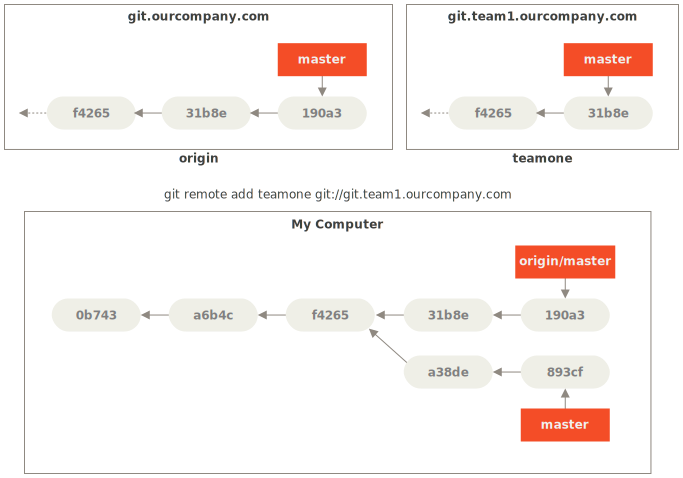
\includegraphics[width=\textwidth,height=0.5\textheight,keepaspectratio]{remote-branches-4}
    \caption{
        Adding another server as a remote\footnote{
            3.5 Git Branching - Remote Branches
            (\url{https://git-scm.com/book/en/v2/Git-Branching-Remote-Branches})
        }
    }
\end{figure}
\end{frame}

\begin{frame}{Remote Branches}{\sectiontitle}
\begin{figure}
    \centering
    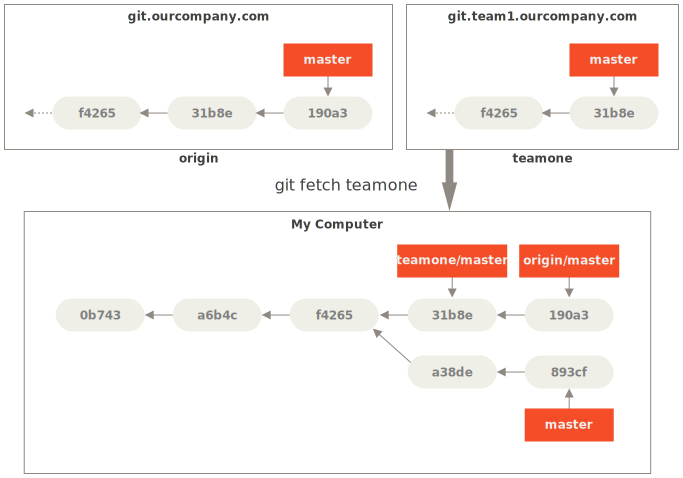
\includegraphics[width=\textwidth,height=0.5\textheight,keepaspectratio]{remote-branches-5}
    \caption{
        Remote-tracking branch for \texttt{teamone/master}\footnote{
            3.5 Git Branching - Remote Branches
            (\url{https://git-scm.com/book/en/v2/Git-Branching-Remote-Branches})
        }
    }
\end{figure}
\end{frame}

\begin{frame}[fragile]{Push Your Changes}{\sectiontitle}
\begin{itemize}
    \item Transfering your changes to a remote is called \emph{pushing}
    \item Your local branches are not automatically pushed to the remote(s)
    \item You need to push your local branches or tags to a remote server, where you have write access
\end{itemize}
\end{frame}

\begin{frame}[fragile]{Push Your Changes}{\sectiontitle}
\begin{block}{\texttt{git push <remote> <branch>}}
\begin{minted}[bgcolor=LightGray,fontsize=\footnotesize]{text}
$ git push origin serverfix
Counting objects: 24, done.
Delta compression using up to 8 threads.
Compressing objects: 100% (15/15), done.
Writing objects: 100% (24/24), 1.91 KiB | 0 bytes/s, done.
Total 24 (delta 2), reused 0 (delta 0)
To https://github.com/schacon/simplegit
 * [new branch]      serverfix -> serverfix
\end{minted}
\begin{itemize}
    \item This is equivalent to \\
          \verb|git push origin serverfix:serverfix|
    \item You can also push to a remote branch with a different name:
          \verb|git push origin serverfix:awesomebranch|
\end{itemize}
\end{block}
\end{frame}

\begin{frame}[fragile]{Tracking Branches}{\sectiontitle}
\begin{minted}[bgcolor=LightGray,fontsize=\footnotesize]{text}
$ git checkout -b serverfix origin/serverfix
Branch serverfix set up to track remote branch serverfix from origin.
Switched to a new branch 'serverfix'
\end{minted}
\begin{block}{Tracking Branches}
\begin{itemize}
    \item Checking out a local branch from a remote-tracking branch
          automatically creates \emph{tracking branch}
    \item A \emph{tracking branch} tracks an \emph{upstream branch}
    \item \verb|git checkout -b <branch> <remote>/<branch>| creates a local
          branch from the remote branch. They point to the same commit.
    \item The \emph{upstream branch} is read-only in the local repository
\end{itemize}
\end{block}
\end{frame}


%%%%%%%%%%%%%%%%%%%%%

\newsection{Workflows}
\begin{frame}{Branching Workflows}{\sectiontitle}
\begin{block}{Long-Running Branches}
\begin{figure}
    \centering
    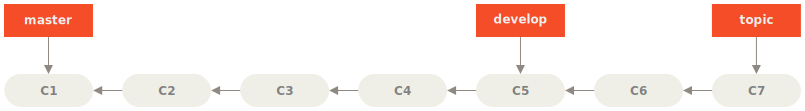
\includegraphics[width=\textwidth,height=0.5\textheight,keepaspectratio]{lr-branches-1}
    \caption{
         A linear view of progressive-stability branching\footnote{
            Pro Git: 3.4 Git Branching - Branching Workflows
            (\url{https://git-scm.com/book/en/v2/Git-Branching-Branching-Workflows})
        }
    }
\end{figure}
\end{block}
\end{frame}

\begin{frame}{Branching Workflows}{\sectiontitle}
\begin{block}{Long-Running Branches}
\begin{figure}
    \centering
    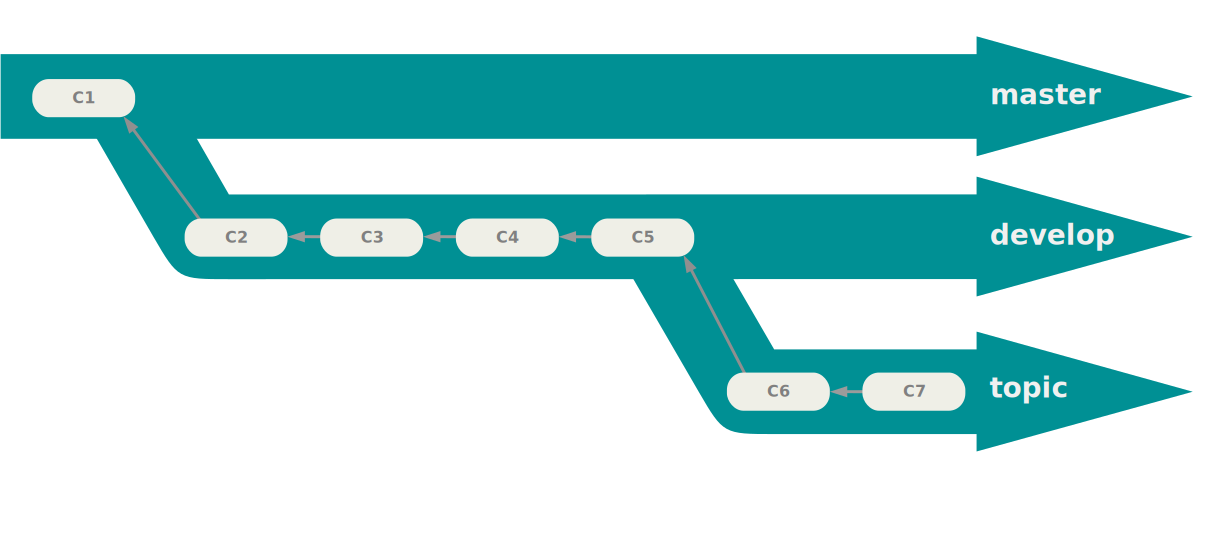
\includegraphics[width=\textwidth,height=0.5\textheight,keepaspectratio]{lr-branches-2}
    \caption{
         A “silo” view of progressive-stability branching\footnote{
            Pro Git: 3.4 Git Branching - Branching Workflows
            (\url{https://git-scm.com/book/en/v2/Git-Branching-Branching-Workflows})
        }
    }
\end{figure}
\end{block}
\end{frame}



\newsection{Github}
\begin{frame}{\sectiontitle}
\begin{block}{ToDo; Or}
Live action role play!
\end{block}
\end{frame}

\newsection{Ressources}
\begin{frame}{Ressources}
\begin{itemize}
    \item Pro Git book: \url{https://git-scm.com/book/en/v2}
    \item Interactive git branching tutorial: \url{https://learngitbranching.js.org/}
    \item The slide sources: \url{https://github.com/iluminat23/git-training}
\end{itemize}
\end{frame}

\end{document}
